\capitulo{3}{Conceptos teóricos}

En este apartado, se van a exponer aquellos conceptos que requieran ser conocidos para comprender cómo se ha realizado el TFG.

\section{Procesamiento de vídeo}
Dado que este proyecto se fundamenta en obtener datos a partir de vídeos, es necesario conocer algunos conceptos básicos de procesamiento de vídeo.

\subsection{Vídeos}
Para que los vídeos sean procesados, es necesario que exista un proceso de lectura de los fotogramas. Además, en ocasiones se desea que los fotogramas sean guardados con el procesado realizado. Esto es lo que se conoce como objetos de vídeo. Un objeto de vídeo puede ser de lectura, cuando se pretende leer los fotogramas del vídeo, o de escritura, cuando se pretende guardar imágenes en forma de vídeo.

Leer un vídeo no requiere un mayor conocimiento más allá de conocer el concepto de fotograma, pero a la hora de escribir un vídeo es necesario conocer el concepto de codificación. Cuando se desea guardar un vídeo o una colección de fotogramas, se puede codificar en varios tipos, lo cual afectará al tipo de extensión del vídeo. Los codificadores más comunes son:
\begin{itemize}
	\item MPEG
	\item H.264
	\item MJPEG
	\item Sorenson
	\item WMV
	\item Ogg Theora
	\item DivX
	\item XviD	
\end{itemize}

Dependiendo del uso que se le vaya a dar al vídeo, conviene utilizar una codificación u otra, dando lugar a extensiones de vídeo diferentes. Estas extensiones definen el tipo de formato del vídeo. Los más comunes son:

\begin{itemize}
	\item AVI
	\item MOV
	\item MP4
	\item ASF
	\item OGG
	\item FLV
	\item MKV
	\item VOB
\end{itemize}

Los vídeos están formados por varias imágenes consecutivas capturadas y reproducidas a cierta velocidad. Esta velocidad se mide en FPS (fotogramas por segundo). Normalmente, los vídeos se capturan a una velocidad de 30 fps y la velocidad de reproducción suele ser la misma, dado que en caso de que una fuese superior a la otra el vídeo se vería acelerado o decelerado. 

En ocasiones, podría resultar interesante acelerar o decelerar una colección de fotogramas procesados, por lo que resulta importante tener en cuenta cuánta aceleración tendrá el objeto de vídeo resultante. Esta aceleración se calcula utilizando la siguiente fórmula:

\begin{equation}
	\text{aceleración} = \frac{\text{fps}_{\text{reproducción}}}{\text{fps}_{\text{captura}}}
\end{equation} 

\subsection{Puntos de la mano}
Una vez comprendidos los conceptos a la hora de procesar vídeos, viene el paso para obtener los puntos de la mano con los que extraer datos que sirvan para realizar una clasificación.

Mediante el objeto de lectura, se van extrayendo todos los fotogramas para procesarlos uno a uno. En cada fotograma, se dibujarán los puntos unidos mediante líneas, tal y como se aprecia en la figura~\ref{fig:puntosmano}. Sin embargo, en este trabajo, sólo serán importantes dos de ellos: el 4 y el 8, ya que son los que representan las puntas de los dedos pulgar e índice respectivamente.

\begin{figure}[h]
	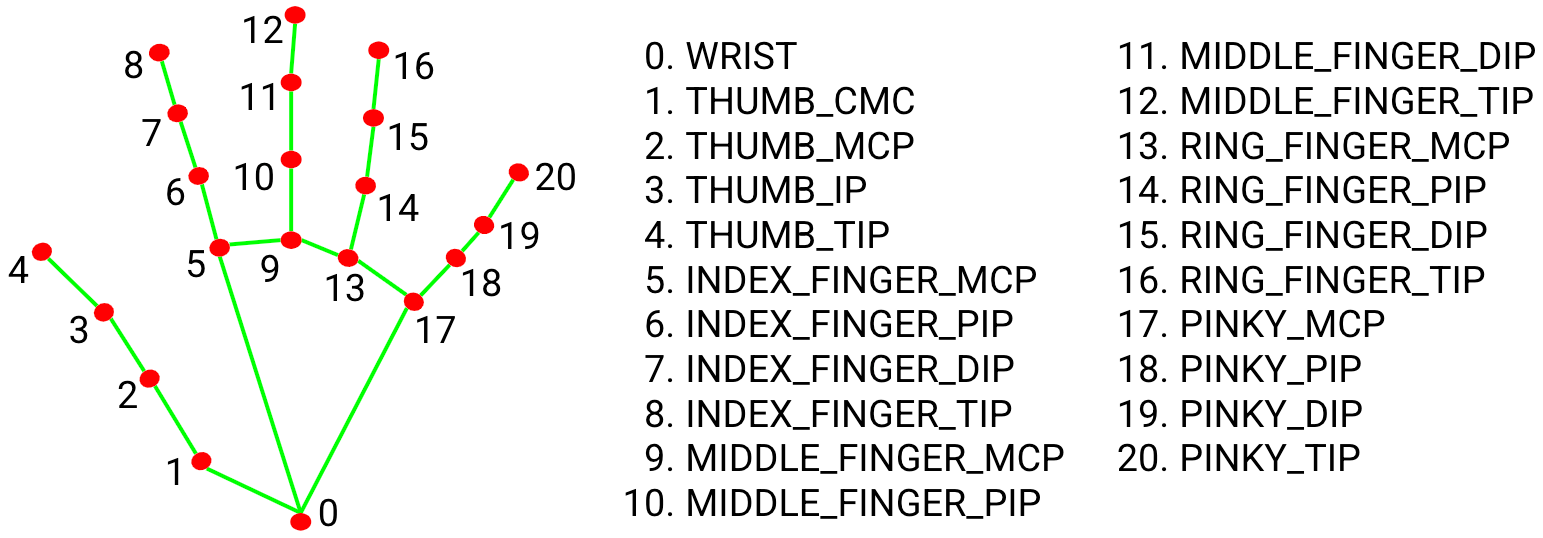
\includegraphics[width=1\textwidth]{puntos_mano}
	\caption{Puntos de la mano y su nombre~\cite{mediapipehands}.}
	\label{fig:puntosmano}
\end{figure}

Una vez establecidos los puntos, se van a obtener las coordenadas de cada fotograma donde están ambos puntos, con el fin de obtener la distancia que los separa en cada instante.

\section{Limpieza de los datos}
Dado que la obtención de los datos del paso anterior no es perfecta, hay que utilizar alguna técnica para eliminar el posible ruido que la biblioteca ha podido ocasionar. Este ruido viene dado porque entre fotogramas, la biblioteca puede detectar el dedo en lugares diferentes sin que este se haya movido, provocando que la amplitud de la pinza se vea afectada.

\subsection{Filtro de Savitzky–Golay}
Este filtrado~\cite{wiki:savgol} ha sido utilizado para eliminar algunas imperfecciones de los datos. Se basa en el cálculo de una regresión polinomial local de grado k con al menos k+1 puntos equiespaciados que determinan el valor de un nuevo punto. Esto hará que los datos varíen y se suavice la gráfica. 

Al dibujar los datos en forma de gráfica, como se observa en la figura \ref{fig:graficadistancias}, se puede apreciar cómo algunas zonas no establecen un único máximo o el máximo podría estar exagerado, por lo que es necesario suavizar esos picos para obtener un solo máximo. 

\begin{figure}[h]
	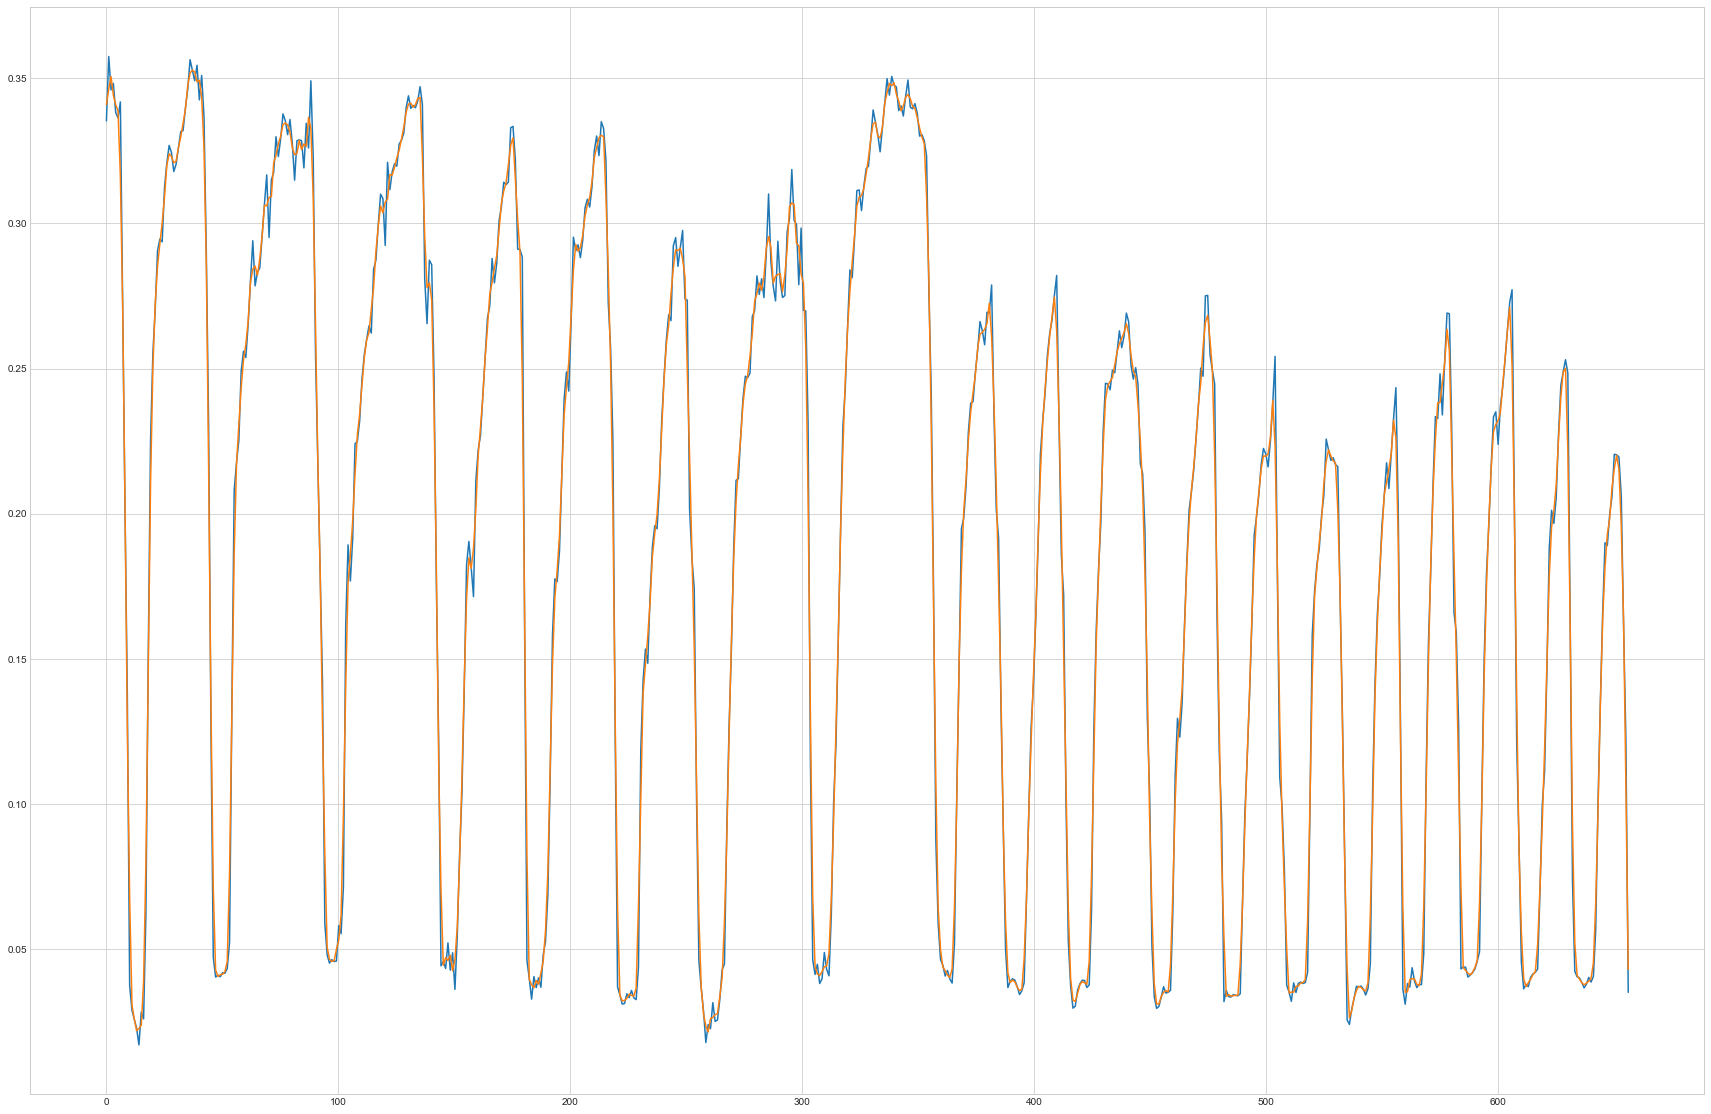
\includegraphics[width=1\textwidth]{grafica_distancias}
	\caption{Representación gráfica de los datos obtenidos en uno de los vídeos sin filtrado (azul) y con filtrado (naranja).}
	\label{fig:graficadistancias}
\end{figure}

La figura \ref{fig:graficadistanciaszoom} muestra uno de los picos de forma ampliada, notándose el suavizado del filtro frente a la gráfica sin suavizar eliminando los picos que producen ruido. Lo ideal sería que la curva fuese lo más perfecta posible, pero el propio pulso de la mano y, sobre todo, la biblioteca que coloca los puntos sobre la mano provocan esas imperfecciones que conviene solucionar. No obstante, aun aplicando el filtrado, no se consigue el resultado ideal, pues el filtrado es únicamente aproximación y una mejora del resultado real.

\begin{figure}[h]
	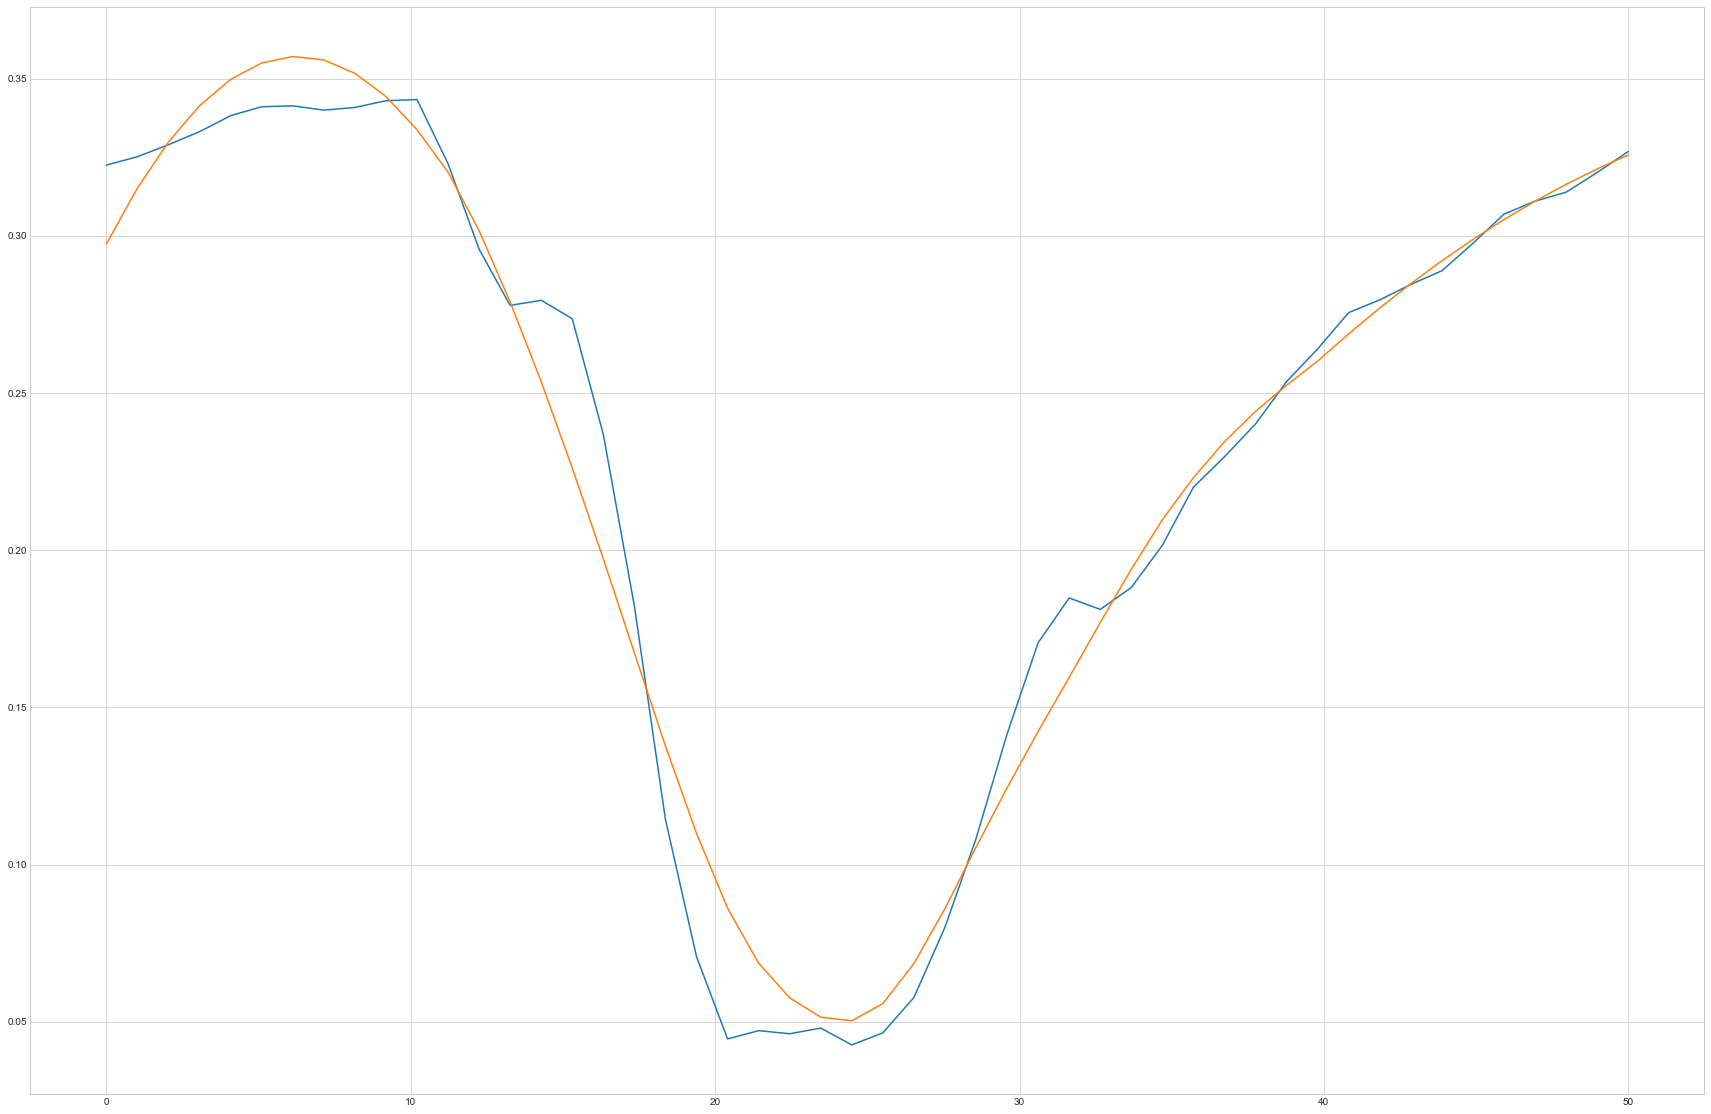
\includegraphics[width=1\textwidth]{grafica_distancias_zoom}
	\caption{Ampliación de uno de los picos donde se aprecia la curva sin suavizar (azul) de la suavizada con el filtro (naranja).}
	\label{fig:graficadistanciaszoom}
\end{figure}

\section{Obtención de características}
A partir de los datos obtenidos en los pasos anteriores, se buscan otros datos que caractericen a los vídeos con el fin de poder realizar una clasificación.

\subsection{Amplitud}
Esta característica es la más evidente ya que, generalmente, la gente con Parkinson ven dificultad a la hora de abrir y cerrar la mano hasta su punto máximo.

Para su extracción, en primer lugar, se ha recogido los máximos y mínimos de la gráfica de los 5 primeros movimientos y de los 5 últimos. Después, estos datos se normalizan para que no afecte la distancia de la mano a la cámara. Esta normalización se obtiene de la siguiente fórmula:

\begin{equation}
	X_{normalizada} = \frac{X_{actual} - X_{mínima}}{X_{máxima}-X_{mínima}}
\end{equation}

Para la extracción de las distancias, tanto la original como la normalizada, tan solo hay que restar el mínimo con el máximo correspondiente. La diferencia de estas distancias de las obtenidas en el apartado anterior es que en estas ahora se tiene en cuenta la distancia entre los dos dedos entre un máximo y un mínimo descontando la pequeña distancia que hay desde la superficie de un dedo hasta el centro donde se encuentra el punto para que la distancia sea más real.

\subsection{Tiempo}
Otra de las características que podrían afectar a una persona que tiene Parkinson es cuánto tardaría en realizar el movimiento de pinza, ya que, en un principio, aquellos que padezcan la enfermedad tardarán más.

Para ello, se ha realizado la diferencia entre un máximo y el mínimo correspondiente, pero en este caso, para obtener el número de fotogramas que hay entre ambos puntos, con el fin de utilizar como unidad temporal el número de fotogramas, ya que, a más lentitud, más fotogramas habrá de diferencia y viceversa.

Sin embargo, esta medida resulta no ser suficiente porque no se tiene en cuenta cuánto se ha abierto la pinza, es decir, alguien que abra la pinza lentamente y hasta la mitad tardará el mismo tiempo que alguien que la abra más rápido y hasta el máximo.

\subsection{Velocidad}
Para solucionar el problema anterior, se puede utilizar la velocidad. Esto es, calcular la distancia recorrida por unidad de tiempo, por lo que dependiendo de cuánto se recorra y en cuánto tiempo una persona tendrá más velocidad o no.

En una primera instancia, una persona que padece Parkinson, dada su reducida movilidad, pese a abrir la pinza hasta su punto máximo, lo más seguro es que lo hiciera de forma más lenta que otra persona sin Parkinson.

Esta velocidad se calcula realizando la división de la diferencia normalizada entre un máximo y un mínimo (i. e. la amplitud ya calculada), entre el tiempo que les separa a ambos puntos (i. e. el tiempo ya calculado).

\subsection{Mano derecha o izquierda}
Como añadido, también se ha tenido en cuenta si la mano es derecha o izquierda. En un principio, podría resultar interesante conocer cuál es la mano que más dificultades tiene a la hora de realizar el movimiento, aunque tampoco resulta fundamental para clasificar. Esta característica no es calculada, sino que viene dada con el vídeo.

\subsection{Sexo}
El sexo de la persona podría servir para clasificar las personas con y sin Parkinson. Como se ha mencionado en la introducción de este documento, el Parkinson es más propenso a aparecer en hombres, por lo que, en primera instancia, podría haber más hombres con Parkinson que mujeres, o lo que es lo mismo, más mujeres sin Parkinson que hombres, lo cual podría ayudar a la hora de clasificar. AL igual que con la mano, esta característica no es calculada, sino que viene dada con el vídeo.

\subsection{Edad}
De forma similar a lo que ocurre con el sexo, el Parkinson es más propenso en personas mayores, de 60 años, por lo que la edad también podría resultar interesante a la hora de clasificar.

Sin embargo, hay que tener cuidado con los ejemplos a la hora de entrenar modelos, ya que el sistema podría aprender que todos los menores de, por ejemplo, 30 años nunca tendrán Parkinson, cuando esto no es cierto. Esta característica tampoco no es calculada, también viene dada con el vídeo.

\section{Minería de datos}
Este punto trata de encontrar patrones en los datos que sirvan para clasificar. Para el problema planteado de predicción, hay que utilizar la clasificación.

La clasificación es una tarea de la minería de datos que realiza un proceso de asignación de una clase u otra dependiendo de los valores que tengan los datos. Extrapolado a este trabajo, esto sería asignar si una persona tiene Parkinson o no dependiendo de las características obtenidas en el punto anterior.

\subsection{Conjunto de ejemplos}
Las características obtenidas son las que conforman el conjunto de datos. Este conjunto de datos será mejor cuantos más ejemplos haya, ya que más opciones podrán abarcar los clasificadores y mejores serán las predicciones.

Los clasificadores se utilizan realizando una separación del conjunto total de los datos. Esta separación da lugar a los datos de entrenamiento y los datos de test:

\begin{itemize}
	\item Conjunto de entrenamiento: constituye la mayor parte de los datos, entre el 70 \% y 80 \% generalmente. Sirve para enseñar al modelo a clasificar el conjunto de datos, indicándole qué casos son de una clase y que casos de otra.
	\item Conjunto de test: Sirve para probar cuánto de bueno es el modelo entrenado con los ejemplos de entrenamiento. Tras las predicciones, se comprobará la clase asignada a cada ejemplo y la clase real y se obtendrán unas precisiones.
\end{itemize}

El conjunto de entrenamiento ha de contener más ejemplos que el conjunto de test debido a que cuanto más ejemplos se ofrezcan al modelo, más probable es que aprenda correctamente. Además, para probar cómo de bueno es un modelo, no son necesarios un alto número de ejemplos.

Es importante que a la hora de evaluar el modelo se utilicen datos que no han sido utilizados para entrenar el modelo, ya que esos ejemplos siempre los acertarían. Debido a esto, es necesario tener estas dos divisiones.

\subsection{Validación cruzada}
La validación cruzada es una técnica que se utiliza a la hora de entrenar y probar modelos de aprendizaje. Se basa en dividir el conjunto de datos en un número de partes y utilizar cada una de las partes como conjunto de test y el resto para entrenar el modelo, tal y como se aprecia en la figura \ref{fig:valcruzada}. Cada una de las partes será utilizada como conjunto de test de forma iterativa.

\begin{figure}[h]
	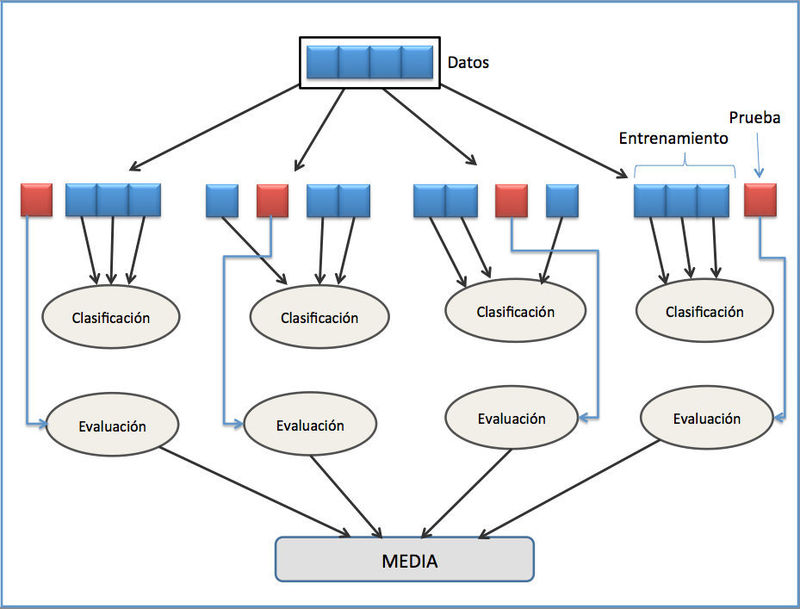
\includegraphics[width=1\textwidth]{validacion_cruzada}
	\caption{Validación cruzada dividendo el conjunto de ejemplos en 4 partes.\cite{wiki:valcruzada}}
	\label{fig:valcruzada}
\end{figure}

Con esto se consigue que la selección de los conjuntos de entrenamiento y test no perjudique al resultado del modelo y se puedan probar más posibilidades de división de los datos.

\subsection{Modelos de clasificación}
Una de las formas más sencillas de encontrar patrones en los datos es utilizando modelos de aprendizaje. Hay varios modelos, y cada uno utiliza una forma de clasificar diferente. Los modelos empleados en este TFG son:
\begin{itemize}
	\item \textbf{Árboles de decisión:} se trata de construir un árbol formado por nodos con condiciones y hojas con clases, para que los datos sean clasificados dependiendo de si cumplen una condición de un nodo o no.
	\item \textbf{Random Forest:} se trata de clasificar los ejemplos utilizando varios árboles de decisión. Estos árboles se construyen utilizando un subconjunto del conjunto total de datos de entrenamiento. Cada árbol predirá una clase, y la más frecuente será la que se le asigne al atributo.
	\item \textbf{k-Nearest Neighbors:} se trata de obtener la clase de los vecinos más cercanos al ejemplo que se trata de clasificar. En este clasificador, no hay un paso previo de entrenamiento, sino que los datos de entrenamiento serán los que contengan los k vecinos más cercanos.
	\item \textbf{Naive Bayes:} se trata de calcular la frecuencia de aparición de los valores de cada característica para poder realizar una clasificación. Esto haría que 
	un ejemplo con ciertos valores se le asigne una clase debido a la probabilidad de aparición de sus valores.
	\item \textbf{Naive Bayes Gaussiano:} es una variante del clasificador Naive Bayes y se trata de utilizar las probabilidades de que aparezcan los valores de, pero acorde con una distribución normal.
	\item \textbf{SVM:} se trata de conseguir un hiperplano que separe los ejemplos que compartan la misma clase del resto. A la hora de clasificar un ejemplo, dependiendo de dónde se encuentre, se le asignará una clase u otra.
\end{itemize}

\section{Evaluación de los resultados}
Una vez utilizado cada modelo, se evalúan cómo de buenos son los resultados para quedarse con el que mejor clasifique. No obstante, en ocasiones podría haber clasificadores que obtengan un 100 \% de precisión, lo cual no es bueno ya que es muy extraño que un clasificador no tenga ningún error en la predicción.
